\documentclass[a4paper, 11pt]{article}
\usepackage[utf8]{inputenc} % Change according your file encoding
\usepackage{graphicx}
\usepackage{url}
\usepackage[margin=1in]{geometry}
\usepackage{caption}
\usepackage{subcaption}
\usepackage{float}

\usepackage[catalan,english]{babel}


%% Estil de Paràgraf
\setlength{\parskip}{4mm}
\setlength{\parindent}{0mm}

%% Estil lletra
\renewcommand{\familydefault}{\sfdefault}


%% Estil de Paràgraf
\setlength{\parskip}{4mm}
\setlength{\parindent}{0mm}

%opening
\title{Seminar Report: Chatty}
\author{Martín Garcia \and Ferran Arau}
\date{\today{}}

\begin{document}

\maketitle

\section{Introducció}

% Introduce in a couple of sentences the seminar and the main topic related to
% distributed systems it covers.

El seminari té com objectiu desenvolupar un sistema de ''chat'' distribuit
utilizant el paradigma client-servidor mitjançant events. Hi ha de dues
implementacions que cal desenvolupar.

En primer lloc els clients envien missatges a un únic servidor i aquest els
distribueix a la resta. 

En segon lloc, cal desenvolupar un sistema més robust ja que la primera
implementació presenta un únic punt de fallada crític, el servidor. Consisteix
en disposar de diverses instàncies ''Servidor'' i que aquestes es comuniquin
entre si. Els clients poden establir conexió amb qualsevol dels servidors i
aquests facilitaran els missatges rebuts a la resta de servidors propagant així
els missatges fins als clients últims.

\section{Feina de laboratori}

% Present the new code that you have added or how you have implemented a
% required functionality by using small Erlang code snippets (you do not need to
% copy\&paste all the code).

A continuació es presenten les dues implementacions del sistema de ''chat''. Es
mostren les diferències entre el codi original i el de producció mitjançant les
eines de ''history'' que proporciona el repositori utilitzat. 

Es pot consultar el codi d'aquesta sessió a
\url{https://github.com/magarcia/SDX/tree/master/S1}


\section{Experiments}

% Describe the experiments you did and provide evidence of the results you got
% (e.g., use screenshots). In addition, you may provide figures or tables with
% experimental results of the system evaluation. For each seminar, we will
% provide you with some guidance on which kind of evaluation you should do.

Per la primera implementació s'ha provat que el ''chat'' era funcional, és a
dir, s'ha vist que diversos clients es podien comunicar entre si. Tots els
clients poden veure tots els missatges.  També s'ha provat de deshabilitar el
servidor. Els resultats han estat els esperats, la comunicació entre els clients
s'ha vist afectada.

A continuació es mostren les imatges que corroboren les proves fetes.

\begin{center} 
    \textbf{Implementació 1}
\end{center}

\begin{figure}[H]
    \centering   
    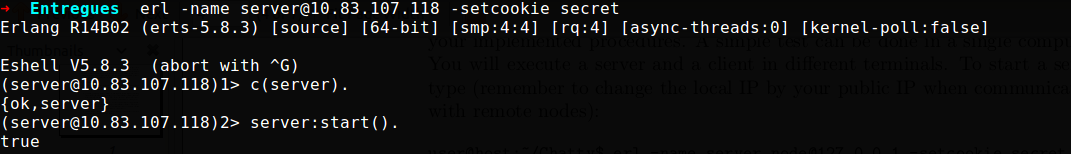
\includegraphics[width=0.8\textwidth]{figures/Server1_start}
    \caption{Servidor \label{fig:Impl1_Server}}
\end{figure}

\begin{figure}[H]
    \centering
	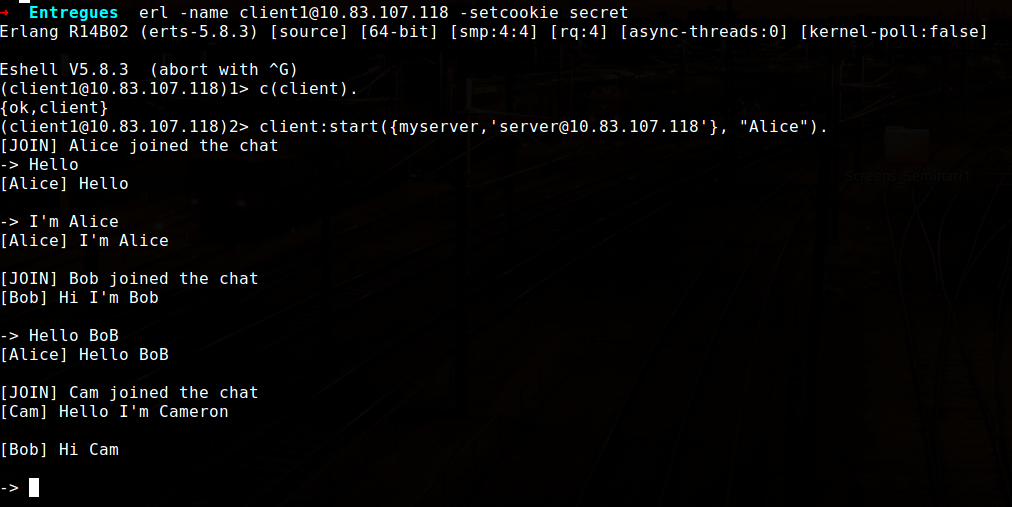
\includegraphics[width=0.8\textwidth]{figures/Server1_Al}
    \caption{Primer Client \label{fig:Impl1_Al}}
\end{figure}

\begin{figure}[H]
    \centering   
	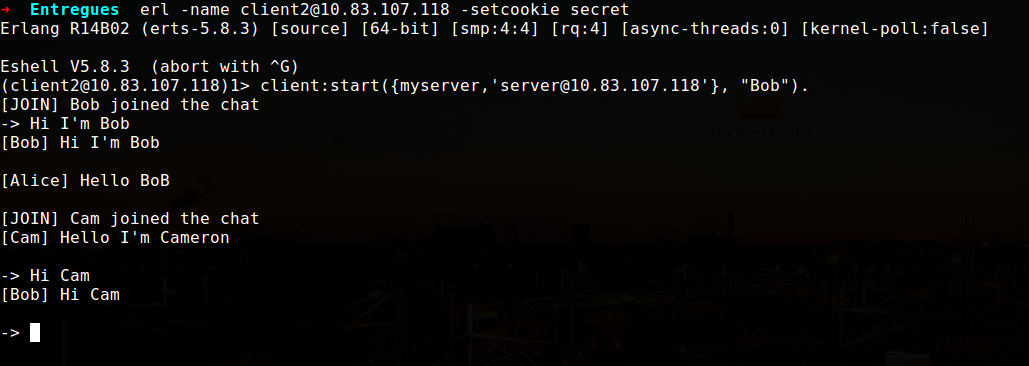
\includegraphics[width=0.8\textwidth]{figures/Server1_Bob}
    \caption{Segon Client \label{fig:Impl1_Bob}}    
\end{figure}    
    
\begin{figure}[H]
    \centering   
	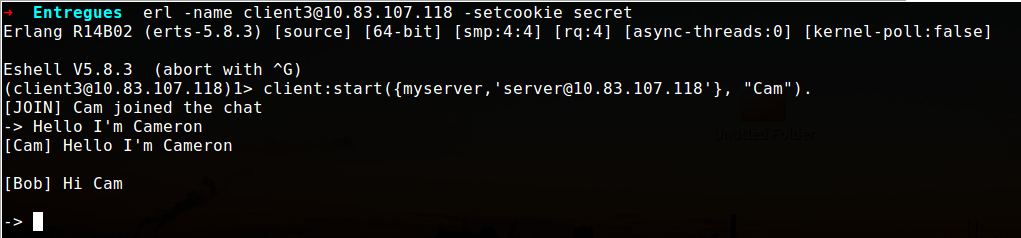
\includegraphics[width=0.8\textwidth]{figures/Server1_Cam}
    \caption{Tercer Client \label{fig:Impl1_Cam}}	
\end{figure}

S'ha pogut veure que els clients Alice, Bob i Cam es poden comunicar entre si. 


La segona implementació consta de dos servidors i quatre clients. Els clients Al i Bob estan conectats al servidor A, el primari. En canvi els clients Cam i Dave es comuniquen mitjançant el servidor secondari, el B.

Si es desconecta el servidor secondari els clients Cam i Dave no poden enviar ni rebre events de manera que queden desconectats del ''chat''. 

A continuació es presenten les imatges que certifiquen les comunicacions entre els diferents clients. 

\begin{center} 
    \textbf{Implementació 2}
\end{center}

\begin{figure}[H]
	\centering
    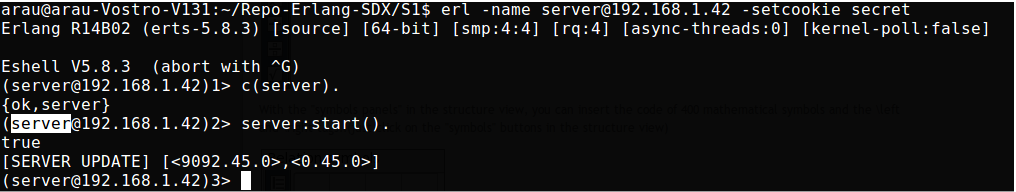
\includegraphics[width=0.8\textwidth]{figures/ServerA}
    \caption{Servidor primari \label{fig:firstserver}}    
\end{figure}

\begin{figure}[H]
	\centering
    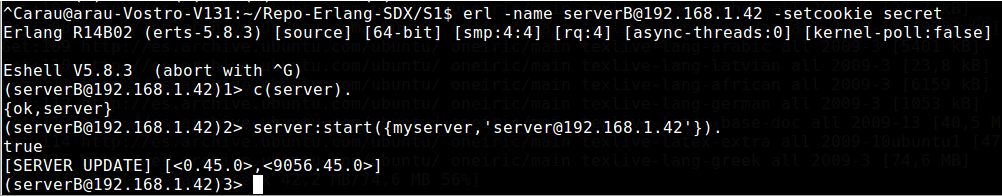
\includegraphics[width=0.8\textwidth]{figures/ServerB}
    \caption{Servidor secondari \label{fig:secondserver}}    
\end{figure}

\begin{figure}[H]
	\centering
    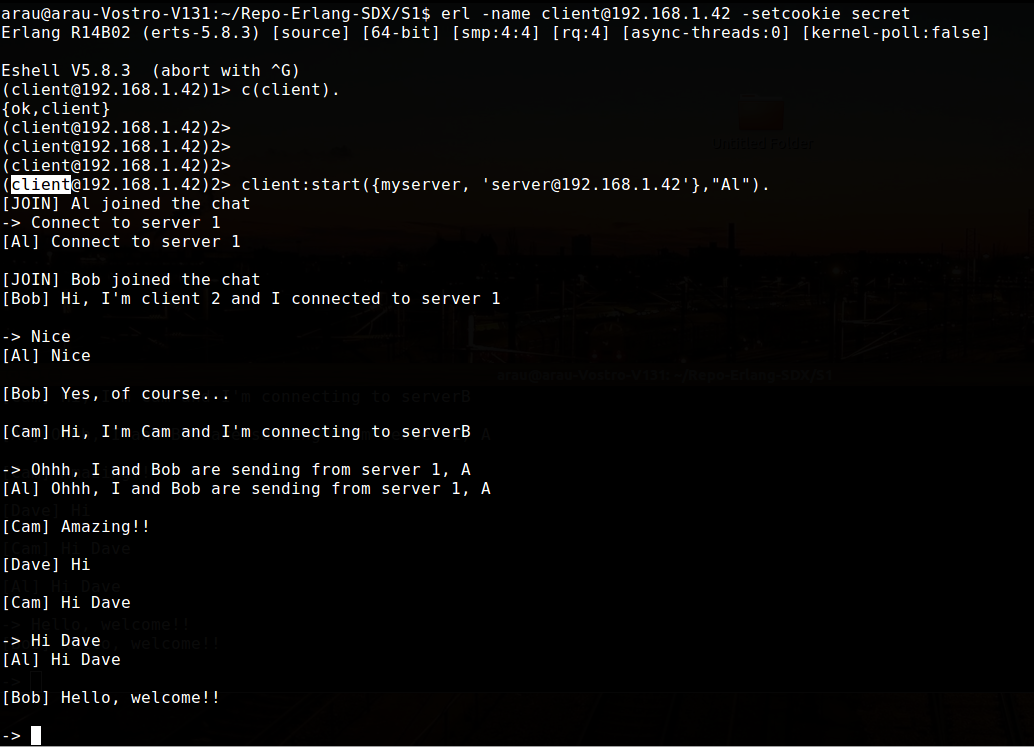
\includegraphics[width=0.8\textwidth]{figures/Al}
    \caption{Client 1 \label{fig:firstclient}}    
\end{figure}
    
\begin{figure}[H]
	\centering
    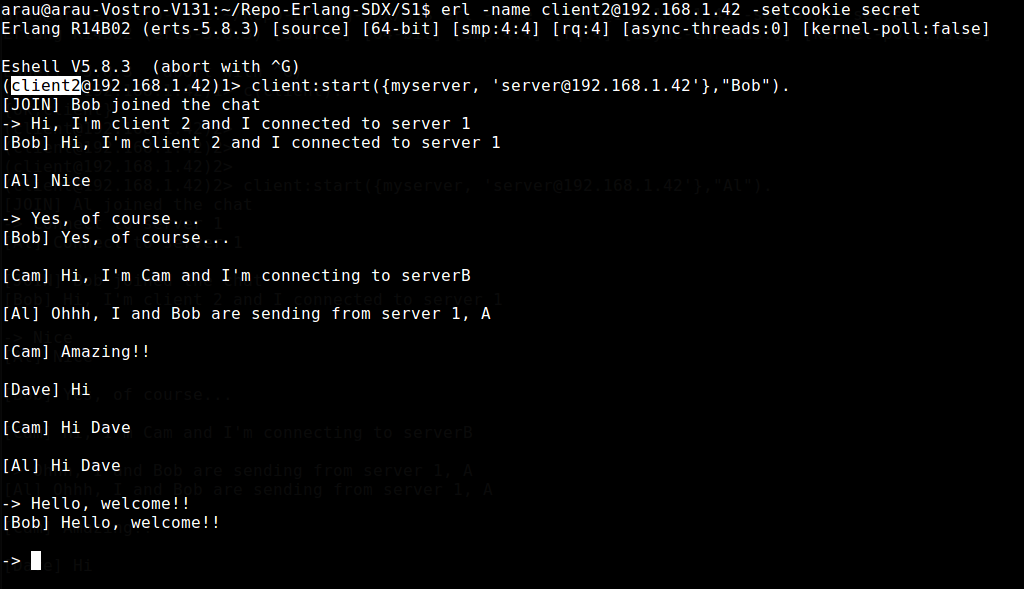
\includegraphics[width=0.8\textwidth]{figures/Bob}
    \caption{Client 2 \label{fig:secondserver}}    
\end{figure}

\begin{figure}[H]
	\centering
    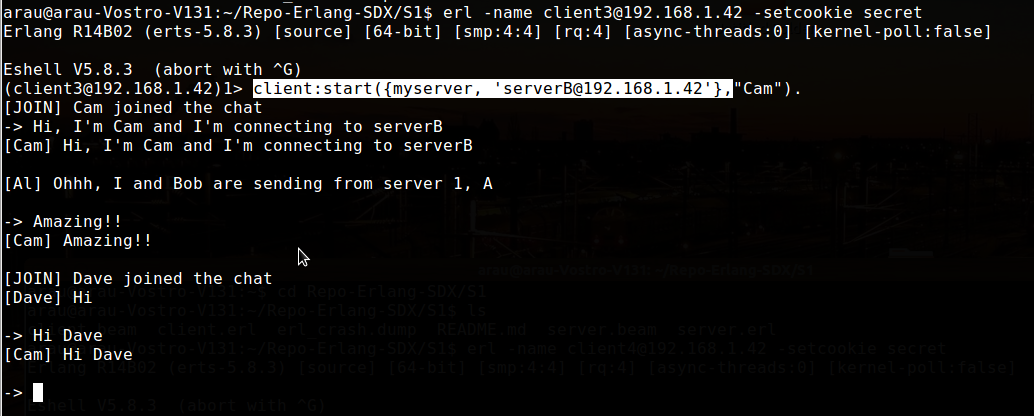
\includegraphics[width=0.8\textwidth]{figures/Cam}
    \caption{Client 3 \label{fig:thirdserver}}    
\end{figure} 
    
\begin{figure}[H]
	\centering
    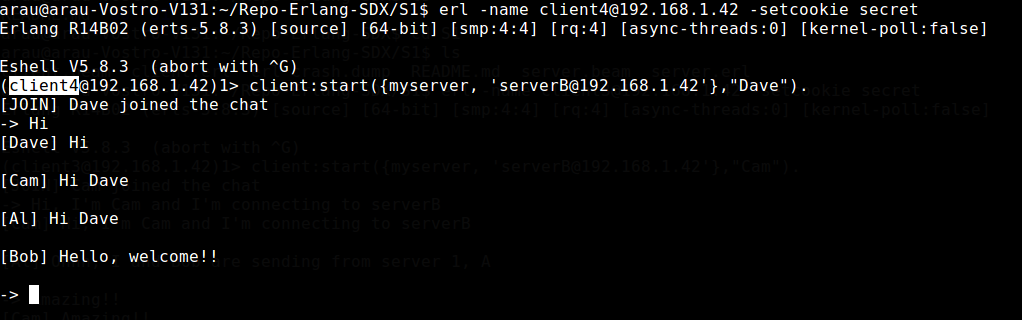
\includegraphics[width=0.8\textwidth]{figures/Dave}
    \caption{Client 4 \label{fig:fourthserver}}    
\end{figure}    

S'ha pogut veure que tots els clients es poden comunicar entre si, malgrat es conecten amb servidors diferents.
Es pot concluïr que els servidors desenvolupen la funció de relay correctament. 

\section{Open questions}

% Try to answer all the open questions in the documentation. When possible, do
% experiments to support your answers.

Implementació 1

El disseny del sistema presenta diverses deficiències. En primer lloc la topologia de l'aplicació presenta un únic punt de fallada, és a dir, tot el sistema queda inutilitzat en el cas que el servidor esdevingui inoperatiu. 

En segon lloc, no permet escalar instàncies de servidor segons el número de peticions. Si es publiquen més events, concurrents, dels que el servidor pot assumir, els missatges es perderan.
Es pot afirmar que el servidor és un coll d'ampolla i que la implementació 1 no escalaria correctament en nombre de clients. 

Els missatges són enviats sense metadades, per tant, no es pot controlar l'ordre d'aparició dels missatges. Tan aviat arriben els missatges el servidor, aquest els propaga. Els clients poden tenir latències de comunicació diferents i per tant dos missatges enviats al mateix temps des de processos erlang diferents mai arribaran a la resta de clients al mateix temps. A més el llenguatge garanteix que l'ordre de missatges es preservar\`a sempre que ambdos missatges provinguin de la mateixa inst\`ancia d'erlang.

Existeixen diferents solucions que permetrien que els missatges es mostressin amb l'ordre en que han estat generats, totes elles requereixen que hi hagi més transferència de dades i per tant que es s'evolucioni el codi del seminàri. 

Per últim dir que la implementació del sistema de ''chat'' no disposa de comunicació transaccional. No hi ha verificació de que els missatges arribin de manera consisten al seu destinatari. També cal remarcar que si un usuari abandona el ''chat'' i si torna a unir més tard, tots els missatges rebuts durant l'absència no seran entregats. 
De nou es pot solucionar aquesta restricció afegint complexitat en el servidor. Caldria, per exemple, implementar un sistema de bústies. 

Implementació 2

En el cas que un servidor esdevingui inoperatiu, tots els seus clients es veuran aïllats. No podran rebre ni enviar missatges. Tot i això, la resta de servidors amb els respectius clients seguiran funcionant.
Una possible solució seria implementar un \textit{failover} autom\`atic, en el qual els clients tinguessin una llista dels servidors disponibles i s'hi puguessin conectar en cas de necessitat.

L'ordre dels missatges no es pot garantir pels mateixos motius que s'han exposat per l'implementació 1.

La segona implementació presenta punts de millora respecte la primera. Permet escalar horitzontalment instàncies de servidor per tal de repartir la càrrega de peticions o per \textit{conectar} diferents grups de clients. També millora en el fet que segmenta els clients, és a dir, permet agrupar-los. Aquest fet aporta robustès en el sistema distribuit ja que es poden migrar grups sencers entre servidors si s'escau. 
També cal remarcar que la segona implementació aporta més fiabilitat al sistema. Afegint servidors es garanteix que si un d'ells falla tot el clúster no es veurà afectat. El servei es veurà degradat, però gran part dels clients seguiran funcionant. 


\section{Personal Opinion}

% Your personal opinion of the seminar, including whether it should be included
% in next year's course or not.


\end{document}

